\documentclass[11pt]{article}
\usepackage[margin=1in]{geometry}
\usepackage[T1]{fontenc}
\usepackage{lmodern}
\usepackage{amsmath,amssymb}
\usepackage{booktabs}
\usepackage{graphicx}
\usepackage[numbers,sort&compress]{natbib}
\usepackage{xcolor}
\usepackage[colorlinks=true,linkcolor=blue!50!black,citecolor=blue!50!black,urlcolor=blue!50!black]{hyperref}
\graphicspath{{../figures/}}
\newcommand{\todo}[1]{\textcolor{red!70!black}{[TODO: #1]}}

\title{What Does a Mixed-Rank LoRA Router Learn?\\
\large Task-specific routing, but no generalization gain over a smaller plain LoRA}
\author{Author names withheld}
\date{Draft, October 2026}

\begin{document}
\maketitle

\begin{abstract}
Mixture-of-experts variants of LoRA promise to adapt capacity to the input: a learned gate
mixes several low-rank adapters per token and per layer. We test a mixed-rank version (experts of
rank 8, 16 and 32, dense per-token gating in every layer) on Qwen2.5-0.5B fine-tuned jointly on
eight tasks, against plain LoRA baselines of matched and smaller size, with five seeds per arm.
Two questions guide the study. \textbf{Efficiency:} on in-distribution validation data the gated
model is the best arm, but on the official test splits it is not: a plain rank-32 LoRA with half
of its trainable parameters reaches a lower test loss ($0.7770$ vs.\ $0.7794$), and test loss is
U-shaped in adapter size while validation loss keeps improving, i.e.\ the extra capacity fits the
training distribution rather than generalizing. \textbf{Interpretability:} the router does learn
something real. Its routing is strongly task-dependent (the task explains 67--86\% of the gate
variance, rising with depth), reproducible across seeds (correlation $0.90$ between seeds' task
$\times$ layer maps, vs.\ $0.13$ for frozen random gates), and faithful for the largest expert
(removing it hurts most the tasks that route to it). But it contradicts the motivating intuition:
harder, generative tasks are routed to \emph{smaller} experts and easy classification tasks to the
largest one. Expert knockouts further reveal that adapting the middle layers hurts GSM8K in every
architecture we tested, a property of multi-task LoRA rather than of gating.
\end{abstract}

\section{Introduction}
Low-rank adaptation (LoRA) \citep{hu2022lora} fine-tunes a frozen language model by adding a
trainable low-rank update to its weight matrices. Its rank is a single global budget, while
tasks, tokens and layers plausibly need different amounts of adaptation. Mixture-of-experts
routing \citep{shazeer2017moe,fedus2022switch} and adaptive rank allocation
\citep{zhang2023adalora} suggest a natural extension: give each layer several LoRA experts of
\emph{different} ranks and let a learned gate decide, per token, how much of each to use. Similar
LoRA mixtures have been proposed \citep{dou2023loramoe,wu2024mole}; the mixed-rank variant adds an
appealing interpretability hook, because the gate weight on each expert can be read as the
\emph{adaptation capacity} the model chooses to spend.

We ask two questions:
\begin{itemize}
  \item \textbf{Q1 (efficiency).} Is a gated mixture of rank-8/16/32 experts as good as a single
        LoRA with the same number of trainable parameters, or better?
  \item \textbf{Q2 (interpretability).} Does the routing mean something: does it depend on the
        task and the layer, is it reproducible, does it follow task difficulty (harder tasks to
        bigger experts), and is it faithful to what each expert actually contributes?
\end{itemize}

\paragraph{Findings.} (i) The gated model wins on in-distribution validation data but not on the
official test splits, where a plain rank-32 LoRA with half the parameters is the best arm
(Section~\ref{sec:q1}). (ii) The routing is task-specific, reproducible and partly faithful, but
it inverts the difficulty intuition and reflects output format more than difficulty
(Section~\ref{sec:q2}). (iii) Per-task knockouts find that middle-layer adaptation hurts GSM8K in
gated and plain LoRA alike (Section~\ref{sec:pertask}).

\section{Method}
\label{sec:method}
\paragraph{Mixed-rank gated LoRA.} For every transformer layer $\ell$ and every target linear map
$W$ of that layer, we attach $E=3$ LoRA experts $(A_e, B_e)$ of ranks $r_e \in \{8, 16, 32\}$
with $\alpha_e = 2 r_e$. A per-layer gating network (two-layer MLP, hidden size 256, GELU,
dropout 0.1) reads the layer's normalized input $h_t$ for token $t$ and outputs a dense softmax
$g_{t,\ell} \in \Delta^{E-1}$ (no top-$k$). The adapted output is
\begin{equation}
  y_t = W x_t + E \sum_{e=1}^{E} g_{t,\ell,e}\, \frac{\alpha_e}{r_e}\, B_e A_e x_t ,
\end{equation}
where the factor $E$ makes uniform routing equivalent to a plain LoRA of rank $\sum_e r_e = 56$.
The gate is shared by the seven target maps of the layer (attention $q,k,v,o$ and MLP
gate/up/down projections). Two auxiliary losses are added, both warmed up over the first 10\% of
training: the Switch load-balancing loss \citep{fedus2022switch} (weight $10^{-3}$) and the mean
gate entropy (weight $10^{-2}$).

\paragraph{Arms.} Besides the gated model we train: \textbf{LoRA r66}, plain LoRA matched in
trainable parameters (36.29M vs.\ 36.32M for the gated model, gates included); \textbf{LoRA r56},
plain LoRA with rank $8{+}16{+}32$, which is exactly the gated model with routing switched off;
\textbf{LoRA r8/r16/r32}, a rank curve; and four controls: \textbf{equal ranks} (19/19/18),
\textbf{last quarter} (gates only in layers 18--23, uniform elsewhere), \textbf{global gate} (one
gate shared by all layers, with a layer embedding) and \textbf{frozen random gate} (random gates
never trained, rescaled per layer at initialization so that their top-1 weight matches the
trained gates' 0.65).

\section{Experimental setup}
\label{sec:setup}
\paragraph{Model and data.} Qwen2.5-0.5B \citep{qwen2025qwen25} (24 layers), frozen, fine-tuned
jointly on eight tasks: SQuAD \citep{rajpurkar2016squad}, IMDB \citep{maas2011imdb}, CoNLL-2003
\citep{tjong2003conll}, WikiText \citep{merity2016wikitext}, GSM8K \citep{cobbe2021gsm8k}, XSum
\citep{narayan2018xsum}, CommonsenseQA \citep{talmor2019commonsenseqa} and MNLI
\citep{williams2018mnli}, sampled with fixed weights (0.10--0.15 per task) from at most 20k
training examples per task. Every task is cast as prompt $\rightarrow$ answer text and the loss is
computed on answer tokens only.

\paragraph{Training.} 5000 optimizer steps of 32 sequences (max length 512), AdamW, cosine
schedule with 10\% warmup, fp16 mixed precision with fp32 adapters, identical for every arm.
The learning rate was chosen by a sweep on validation loss for the gated model and LoRA r66
(Appendix~\ref{app:lr}); $5\times10^{-5}$ was best for both and is used for every arm.

\paragraph{Evaluation.} \emph{Validation}: a held-out 5\% of the training data (500 examples
per task, same distribution as training). \emph{Test}: the official evaluation split of each
dataset (1000 examples per task). The main metric is the mean over the eight tasks of the
per-token answer loss (macro answer loss), measured at the last step. Generation is evaluated with
greedy decoding: GSM8K final-number accuracy and XSum ROUGE-L (500 examples each). Main arms use
five seeds; controls three; the global gate one.

\section{Q1: The gated model fits better, a smaller LoRA generalizes better}
\label{sec:q1}
\begin{table}[t]
\centering
\caption{Macro answer loss (mean $\pm$ s.d.\ over seeds; number of seeds in parentheses) at LR
$5\times10^{-5}$. Params: trainable parameters. Generation: GSM8K accuracy and XSum ROUGE-L. Best
mean per column in bold. $^\dagger$Gates frozen (not trained).}
\label{tab:q1}
\begin{tabular}{lrcccc}
\toprule
Arm & Params & Validation & Test & GSM8K & XSum \\
\midrule
Gated 8/16/32 (5) & 36.3M & $\mathbf{0.7685 \pm 0.0011}$ & $0.7794 \pm 0.0019$ & 0.350 & 0.254 \\
LoRA r66 (5)      & 36.3M & $0.7715 \pm 0.0009$ & $0.7802 \pm 0.0013$ & 0.346 & \textbf{0.257} \\
LoRA r56 (5)      & 30.8M & $0.7704 \pm 0.0009$ & $0.7793 \pm 0.0016$ & 0.349 & 0.256 \\
LoRA r32 (5)      & 17.6M & $0.7704 \pm 0.0009$ & $\mathbf{0.7770 \pm 0.0012}$ & 0.350 & 0.252 \\
LoRA r16 (5)      &  8.8M & $0.7736 \pm 0.0005$ & $0.7785 \pm 0.0006$ & \textbf{0.360} & 0.249 \\
LoRA r8 (1)       &  4.4M & $0.7790$ & $0.7827$ & 0.358 & 0.248 \\
\midrule
Equal ranks 19/19/18 (3) & 36.3M & $0.7705$ & $0.7781$ & 0.337 & 0.256 \\
Last quarter only (3)    & 32.2M & $0.7697$ & $0.7783$ & 0.346 & 0.252 \\
Global gate (1)          & & $0.7687$ & $0.7793$ & 0.342 & 0.255 \\
Frozen random gate (3)   & 30.8M$^\dagger$ & $0.7729$ & $0.7816$ & 0.347 & 0.256 \\
\bottomrule
\end{tabular}
\end{table}

\begin{figure}[t]
\centering
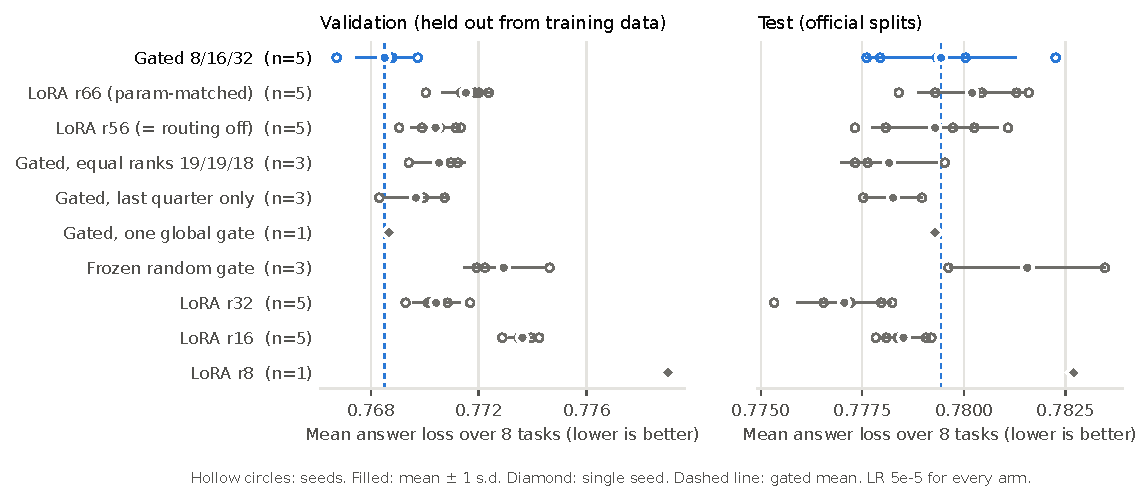
\includegraphics[width=\linewidth]{fig1_q1_losses.pdf}
\caption{Validation (left) and test (right) macro answer loss per arm. The gated model leads on
validation, but on test the arms overlap within seed noise and LoRA r32 is lowest.}
\label{fig:q1}
\end{figure}

Table~\ref{tab:q1} and Figure~\ref{fig:q1} give the main comparison.
\textbf{On validation the gated model is the best arm}, ahead of the parameter-matched LoRA r66
by $0.0030$ (Welch $t=-4.7$, five seeds each). \textbf{On test the advantage disappears}
($-0.0008$, $t=-0.75$) and the gated model ties LoRA r56, i.e.\ itself with routing switched off
($+0.0001$). Generation metrics are indistinguishable across arms.

\textbf{The best test loss belongs to plain LoRA r32}, with 17.6M trainable parameters against
36.3M: $0.7770 \pm 0.0012$, lower than the gated model ($-0.0024$, $t=-2.4$), LoRA r66
($-0.0032$, $t=-3.9$) and LoRA r56 ($-0.0023$, $t=-2.6$). Along the rank curve, test loss is
U-shaped (r8 $0.7827$, r16 $0.7785$, r32 $0.7770$, r56 $0.7793$, r66 $0.7802$) while validation
loss improves up to r32 and then stays flat or drifts. Capacity beyond rank~32 therefore fits the
training distribution without improving generalization, and the gated model, with the largest
budget, behaves like the large adapters. The learning rate was tuned for the gated model and r66,
not for r32, which can only favor them.

\paragraph{Where the validation gain goes.} Per task (Appendix~\ref{app:pertask}), the gated
model's validation advantage over r66 is real on test for CommonsenseQA ($-0.011$ on both splits),
GSM8K ($-0.008$ / $-0.007$) and CoNLL-2003, but it loses on XSum, SQuAD and IMDB on both splits,
and on WikiText the sign flips ($-0.005$ on validation, $+0.005$ on test). The gains and losses
cancel on the official splits.

\section{Q2: What the router learns}
\label{sec:q2}
\begin{figure}[t]
\centering
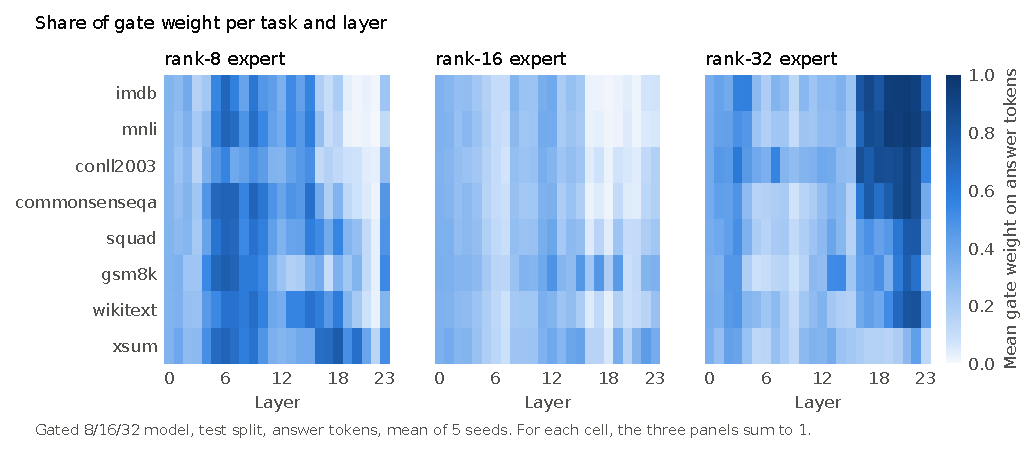
\includegraphics[width=\linewidth]{fig2_routing.pdf}
\caption{Share of gate weight per task (rows) and layer (columns) for each expert, on answer
tokens of the test split, averaged over five seeds.}
\label{fig:routing}
\end{figure}

\paragraph{Routing is task- and layer-specific.} Figure~\ref{fig:routing} shows a consistent
layer structure. In the first four layers the three experts receive similar weight; in layers
4--15 the two small experts together receive most of the weight for every task (0.57--0.87),
with the rank-8 expert alone at 0.42--0.68 in layers 4--11; in layers 16--23 classification-like tasks
(IMDB, MNLI, CoNLL-2003, CommonsenseQA) switch almost entirely to the rank-32 expert (0.70--0.92
of the weight), while XSum keeps most of its weight on the two small experts. The task explains
67\%, 73\% and 86\% of the variance of the gate vector in early, middle and late layers (a
permutation-invariant $\eta^2$), against 50--60\% for frozen random gates, whose weights still
depend on the input but not in a learned way.

\paragraph{Routing is reproducible.} The task $\times$ layer maps of expected rank correlate at
$0.90$ on average between pairs of seeds (minimum $0.83$), against $0.13$ for frozen random gates.
With equal ranks the correlation drops to $0.12$: the experts are interchangeable, so each seed
labels them differently. Mixed ranks break this symmetry, which is what makes the routing
interpretable at all.

\paragraph{Routing inverts the difficulty intuition.} Measuring difficulty by a task's answer
loss, the correlation between difficulty and expected rank across tasks is strongly
\emph{negative} in every seed (Spearman $-0.83$ to $-0.95$): the hardest tasks (WikiText, XSum,
GSM8K) receive the smallest experts. Within a task, harder examples are not routed to bigger
experts either ($\rho$ between $-0.09$ and $-0.01$). The pattern is better explained by output
format: tasks whose answer departs most from free-text continuation (labels, entity tags,
multiple-choice letters) draw on the largest expert in late layers. \todo{test this hypothesis
directly, e.g.\ with format-matched task pairs.}

\begin{figure}[t]
\centering
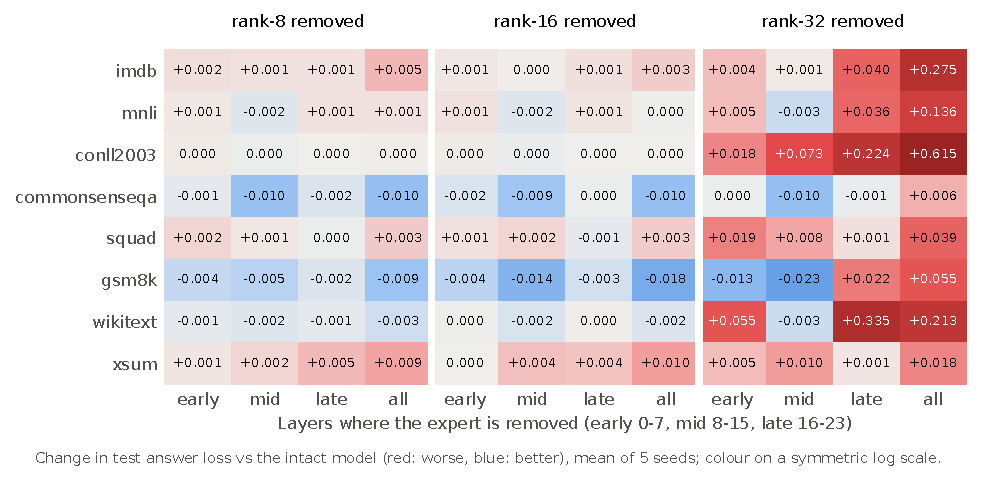
\includegraphics[width=\linewidth]{fig3_knockout.pdf}
\caption{Change in test answer loss when one expert's gate weight is set to zero in a block of
layers (no renormalization), mean of five seeds. Red: worse; blue: better.}
\label{fig:ko}
\end{figure}

\paragraph{Knockouts: the router is faithful for the largest expert.} We remove one expert by
setting its gate weight to zero in a block of eight layers, without renormalizing the others
(Figure~\ref{fig:ko}). Removing the rank-32 expert everywhere raises the macro test loss by
$0.170$, mostly through the late layers ($+0.082$), and the damage follows its routing: across
tasks, the share of weight a task puts on the rank-32 expert predicts how much it suffers when the
expert is removed (Spearman $0.67$ for all layers; $0.57$, $0.38$ and $0.39$ for the early, middle
and late blocks). Removing a small expert barely changes the macro loss ($-0.0005$ and $-0.0018$),
but this average hides opposite per-task effects: XSum needs the small experts ($+0.009$ and
$+0.010$, about half of the $+0.018$ caused by removing the rank-32 expert), whereas GSM8K and
CommonsenseQA \emph{improve} without them ($-0.009$/$-0.018$ and $-0.010$/$-0.010$). With frozen
random gates the work is spread more evenly (rank-32 removal: $+0.047$) and the damage does not
follow the routing (mean $\rho=-0.05$).

\section{Per-task knockouts: middle-layer adaptation hurts GSM8K in every architecture}
\label{sec:pertask}
\begin{table}[t]
\centering
\caption{Test macro answer loss when, for each task, the removal that minimizes that task's
\emph{validation} loss is applied (chosen per seed; scored on test). Gated: six options (none;
rank-8+16 removed from all, early, middle or late layers; rank-32 removed from middle layers).
Plain LoRA: four options (none; whole adapter removed from early, middle or late layers).}
\label{tab:pertask}
\begin{tabular}{lcccc}
\toprule
 & Intact & Per-task removal & GSM8K change & CommonsenseQA change \\
\midrule
Gated 8/16/32 & 0.7794 & \textbf{0.7750} & $-0.023$ & $-0.010$ \\
LoRA r66      & 0.7802 & 0.7769 & $-0.023$ & $-0.004$ \\
LoRA r56      & 0.7793 & 0.7769 & $-0.017$ & $-0.002$ \\
\bottomrule
\end{tabular}
\end{table}
The knockouts suggest that some adaptation is harmful for some tasks. To test this without
selecting on the test set, we choose for each task and seed the removal that minimizes the
\emph{validation} loss, then score it on test (Table~\ref{tab:pertask}). For GSM8K, all five
seeds of all three architectures choose to remove the middle-layer adaptation (for the gated
model, the rank-32 expert in layers 8--15), and test loss drops by $0.017$--$0.023$. The effect is
therefore a property of multi-task LoRA on this model, not of gating; the gate maps only helped to
locate it. The gated model gains a further $0.002$, mostly on CommonsenseQA, which we attribute to
its finer set of removal options. XSum and SQuAD keep every adapter in every seed.

\section{Discussion}
The router behaves as intended in one sense: it learns a stable, task-specific allocation of
adapters across layers, and the weight it gives to the largest expert predicts that expert's
importance. It does not translate into better generalization, for a simple reason visible in the
rank curve: at this scale the bottleneck is not adapter capacity. Test loss is minimized by a
rank-32 LoRA, and every larger budget, including the 36M-parameter gated mixture, fits the
training distribution better while generalizing slightly worse. Mixed ranks matter for
interpretability (they make routing reproducible) more than for accuracy.

\section{Limitations}
One base model (0.5B parameters) and one task mixture; the conclusions may change for larger
models or capacity-bound regimes. \todo{replicate on a second model (Pythia-410M or
SmolLM-360M).} The learning rate was tuned for the gated model and LoRA r66 only; at
$2.5\times10^{-5}$ both reach a lower test loss (0.7764 and 0.7767, two seeds each), so the test
ranking at the tuned rate should be read with that in mind. Controls have three seeds and the
global gate one. Effects are small (a few thousandths of answer loss), comparable to seed noise
for some comparisons; we report seed spreads and uncorrected Welch $t$ statistics. Test metrics
are taken at the last training step; a val-selected checkpoint was not available for every run.

\bibliographystyle{plainnat}
\bibliography{refs}

\appendix
\section{Learning-rate sweep}
\label{app:lr}
\begin{table}[h]
\centering
\caption{Validation macro answer loss by learning rate (number of seeds in parentheses).}
\begin{tabular}{lccccc}
\toprule
 & $2.5\times10^{-5}$ & $5\times10^{-5}$ & $10^{-4}$ & $2\times10^{-4}$ & $4\times10^{-4}$ \\
\midrule
Gated 8/16/32 & 0.7691 (2) & \textbf{0.7685} (5) & 0.7719 (2) & 0.7818 (2) & 0.7929 (2) \\
LoRA r66      & \textbf{0.7708} (2) & 0.7715 (5) & 0.7769 (2) & 0.7886 (2) & 0.8292 (2) \\
\bottomrule
\end{tabular}
\end{table}
The sweep used validation loss; $5\times10^{-5}$ was selected for both arms before the
$2.5\times10^{-5}$ check was run.

\section{Per-task validation vs.\ test}
\label{app:pertask}
\begin{table}[h]
\centering
\caption{Per-task answer loss of the gated model minus the baseline (mean over five seeds;
negative = gated better).}
\begin{tabular}{lrrrr}
\toprule
 & \multicolumn{2}{c}{vs.\ LoRA r66} & \multicolumn{2}{c}{vs.\ LoRA r56} \\
Task & val & test & val & test \\
\midrule
CommonsenseQA & $-0.0107$ & $-0.0106$ & $-0.0048$ & $-0.0048$ \\
CoNLL-2003    & $-0.0033$ & $-0.0023$ & $-0.0037$ & $-0.0031$ \\
GSM8K         & $-0.0084$ & $-0.0069$ & $-0.0002$ & $-0.0000$ \\
IMDB          & $+0.0009$ & $+0.0023$ & $+0.0018$ & $+0.0003$ \\
MNLI          & $-0.0022$ & $-0.0010$ & $-0.0015$ & $-0.0007$ \\
SQuAD         & $+0.0022$ & $+0.0028$ & $-0.0005$ & $-0.0001$ \\
WikiText      & $-0.0053$ & $+0.0054$ & $-0.0077$ & $+0.0069$ \\
XSum          & $+0.0027$ & $+0.0041$ & $+0.0015$ & $+0.0027$ \\
\midrule
Macro mean    & $-0.0030$ & $-0.0008$ & $-0.0019$ & $+0.0001$ \\
\bottomrule
\end{tabular}
\end{table}

\end{document}
